%!TEX root = ../Dimensionieren I.tex

\section{Kerben} % (fold)
	\begin{enumerate}
		\item Plötzliche Querschnittsänderungen (Bohrungen, Nuten, Absätze)
		\item Plötzliche Kraftumlenkungen (Ecken, Schweissnähte)
		\item Steifigkeitsänderungen (Lot, Klebefugen)
		\item Ungewollte Kerben (Poren, Einschlüsse, Risse, Korrosion)
	\end{enumerate}
% section: Kerben (end)
\section{Nennspannung} % (fold)
	\begin{equation*}
		\begin{array}{@{}l@{\quad}r@{\:=\:}l@{\ ,\qquad}r@{\:=\:}l}
			\text{Zug/Druck:} & \sigma_n & \displaystyle\frac{F}{A} & \sigma_{\text{maxK}} & \alpha_{\sigma\text{(Zug)}}\cdot \sigma_n \\[2ex]
			\text{Biegung:} & \sigma_n & \displaystyle\frac{M_B}{W_B} & \sigma_{\text{maxK}} & \alpha_{\sigma\text{(Biegung)}}\cdot \sigma_n \\[2ex]
			\text{Torsion:} & \tau_n & \displaystyle\frac{M_t}{W_p} & \tau_{\text{maxK}} & \alpha_{\tau\text{(Torsion)}}\cdot \tau_n
		\end{array}
	\end{equation*}
	\begin{tightitemize}
		\item[$A$:] durch Kerbe geschwächter Nettoquerschnitt
		\item[$W_B$:] Widerstandsmoment im Nettoquerschnitt
		\item[$W_P$:] polares Widerstandsmoment im Nettoquerschnitt
	\end{tightitemize}
% section: Nennspannung (end)
\section{Formzahl} % (fold)
	Allgemein:
	\begin{equation*}
		\alpha_{\sigma\text{(Zug)}} > \alpha_{\sigma\text{(Biegung)}} > \alpha_{\tau\text{(Torsion)}} > 1
	\end{equation*}
	Formzahl ist \emph{zu berücksichtigen} bei:
	\begin{tightitemize}
		\item spröden Materialien
		\item Glas, Karamik, Grauguss etc.
	\end{tightitemize}
	Formzahl ist \emph{nicht zu berücksichtigen} bei:
	\begin{tightitemize}
		\item duktilen Materialien
		\item Aluminium, Stahl, Kunststoff etc.
	\end{tightitemize}
	
	\subsection{Formzahl für Absatz und Rundnut} % (fold)
		\begin{equation*}
			\alpha_{\sigma,\tau} = 1 + \left( A \frac{r}{t} + 2B \frac{r}{d}\left( 1 + 2 \frac{r}{d}\right)^2 + C \left( \frac{r}{t}\right)^Z \frac{d}{D}\right)^{-1/2}
		\end{equation*}
		mit $t= \frac{1}{2} (D-d)$.
		\begin{center}
			\begin{tabular}{r|lr@{}lr@{}lr@{}lr@{}l}
				\toprule
				& \textbf{Belastung} & \multicolumn{2}{c}{$\boldsymbol A$} & \multicolumn{2}{c}{$\boldsymbol B$} & \multicolumn{2}{c}{$\boldsymbol C$} & \multicolumn{2}{c}{$\boldsymbol Z$} \\
				\midrule
				\multirow{3}{*}{
				\begin{sideways}
					\textbf{Rundnut}
				\end{sideways}
				} & Zug/Druck & 0&.22 & 1&.37 & 0& & 0& \\
				& Biegung & 0&.2 & 2&.75 & 0& & 0& \\
				& Torsion & 0&.7 & 10&.3 & 0& & 0& \\
				\midrule
				\multirow{3}{*}{
				\begin{sideways}
					\textbf{Absatz}
				\end{sideways}
				} & Zug/Druck & 0&.62 & 3&.5 & 0& & 0& \\
				& Biegung & 0&.62 & 5&.8 & 0&.2 & 3& \\
				& Torsion & 3&.4 & 19& & 1& & 2& \\
				\bottomrule
			\end{tabular}
		\end{center}
		\begin{TI}
			\verb=ALPHA(=$A$\verb=,=$B$\verb=,=$C$\verb=,=$Z$\verb=,=$r$\verb=,=$d$\verb=,=$D$\verb=)=
		\end{TI}
	% subsection: Formzahl für Absatz und Rundnut (end)
	\subsection{Formzahl für Absatz mit Freistich} % (fold)
		\begin{center}
			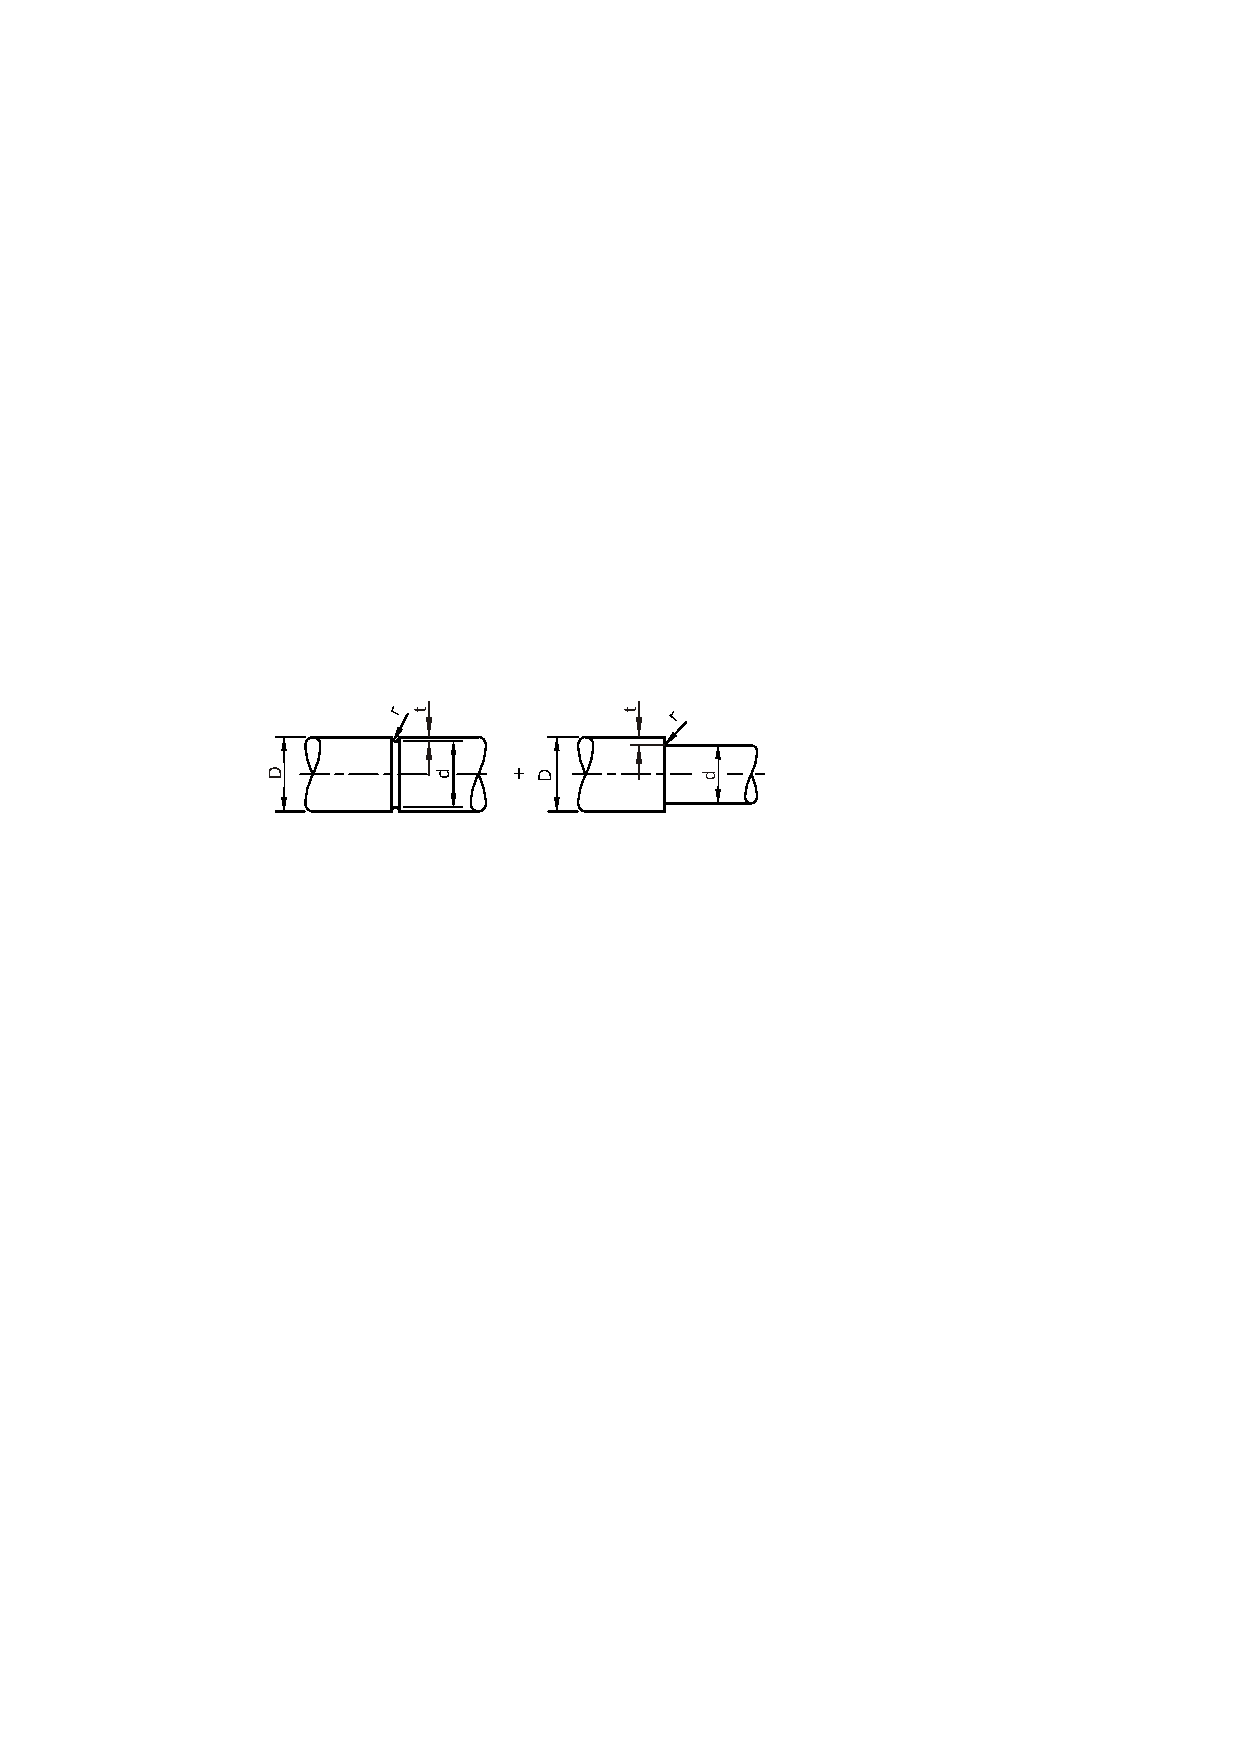
\includegraphics{graphics/freistich_kerbe_1}\\
			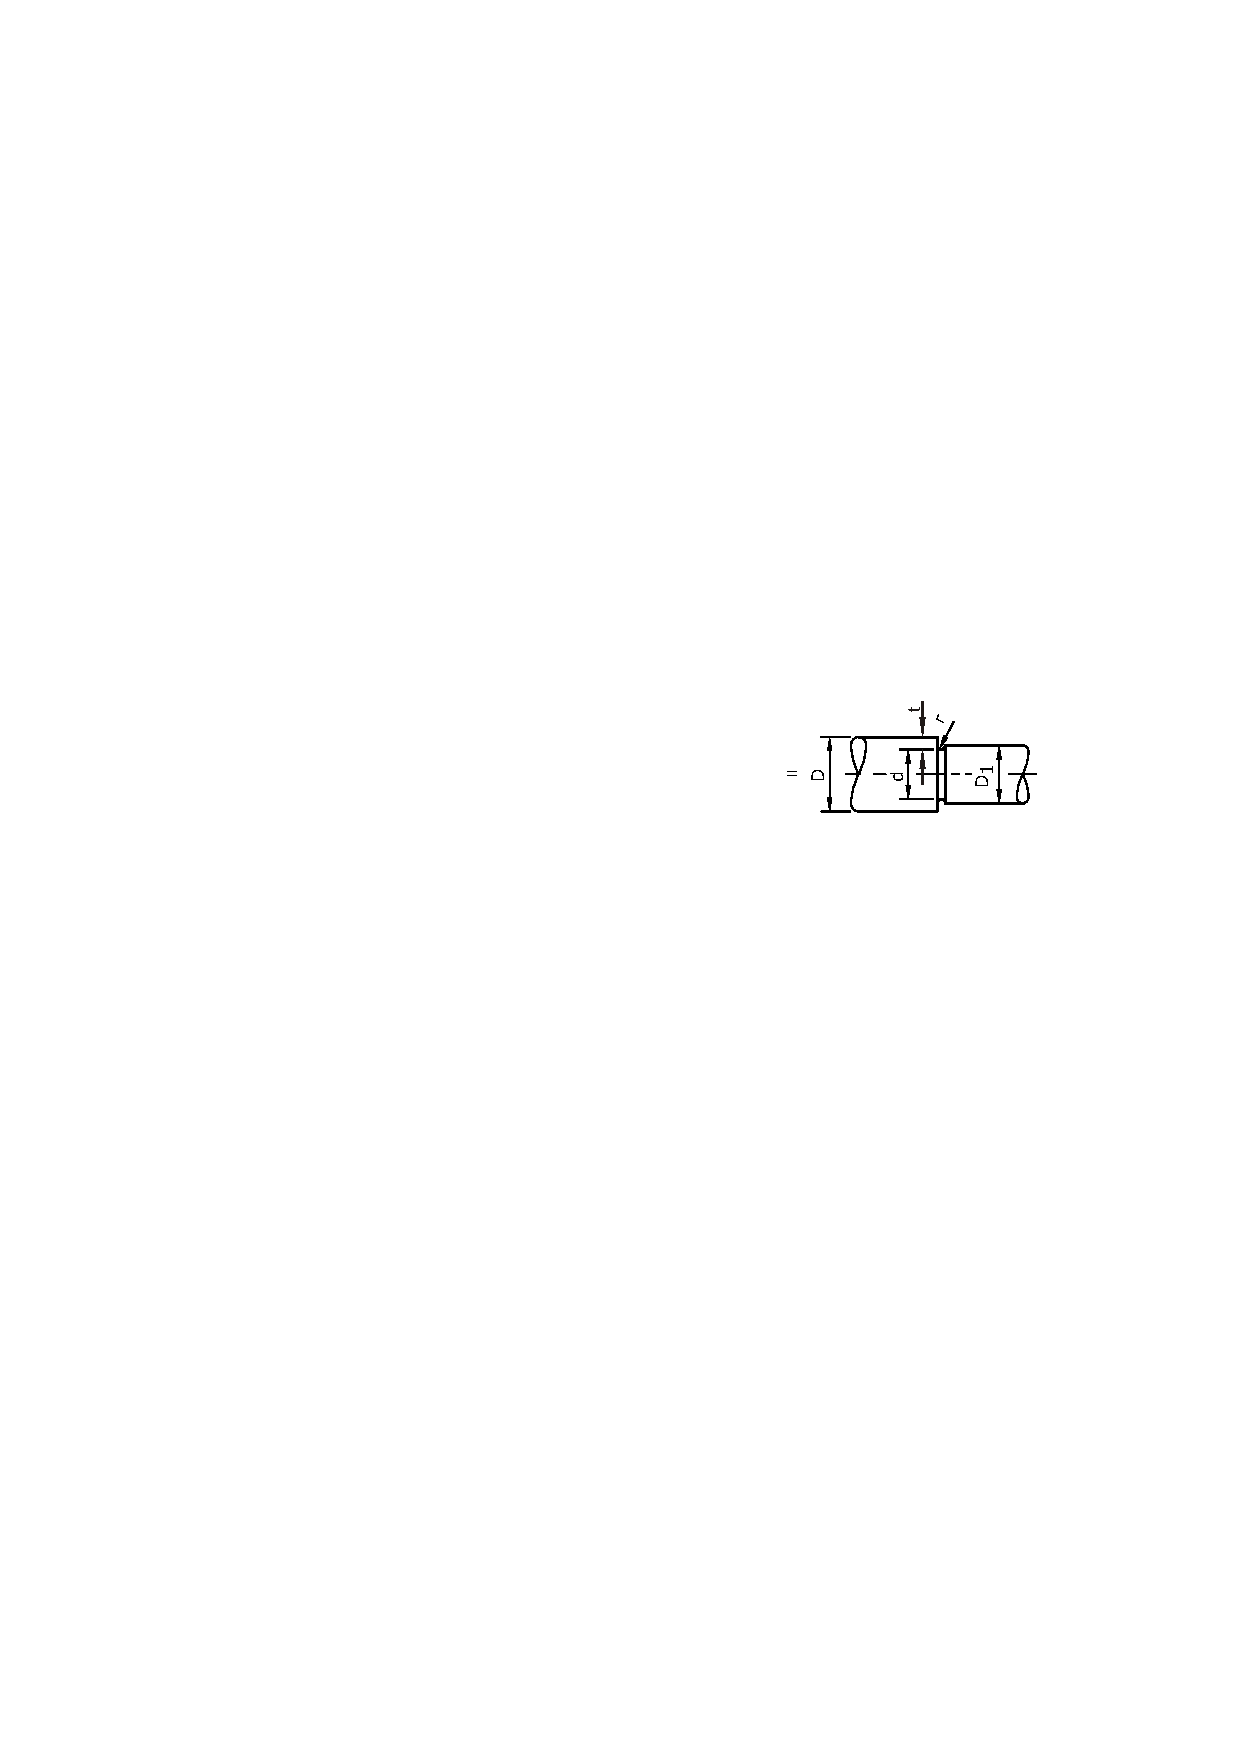
\includegraphics{graphics/freistich_kerbe_2}
		\end{center}
		\begin{equation*}
			\text{Rundnut (R)} + \text{Absatz (A)} = \text{Absatz mit Freistich (F)}
		\end{equation*}
		
		Man kombiniert die Formzahlen einer Rundnut und eines Absatzes folgendermassen:
		\begin{align*}
			\alpha_{\sigma\text{F}} &= (\alpha_{\sigma\text{R}}-\alpha_{\sigma\text{A}}) \cdot \sqrt{\frac{D_1-d}{D-d}} + \alpha_{\sigma\text{A}} \\
			\alpha_{\tau\text{,F}} &= 1.04 \cdot \alpha_{\tau\text{,A}}
		\end{align*}
	% subsection: Formzahl für Absatz mit Freistich (end)
	\subsection{Formzahl für Rundstab mit Querbohrung} % (fold)
		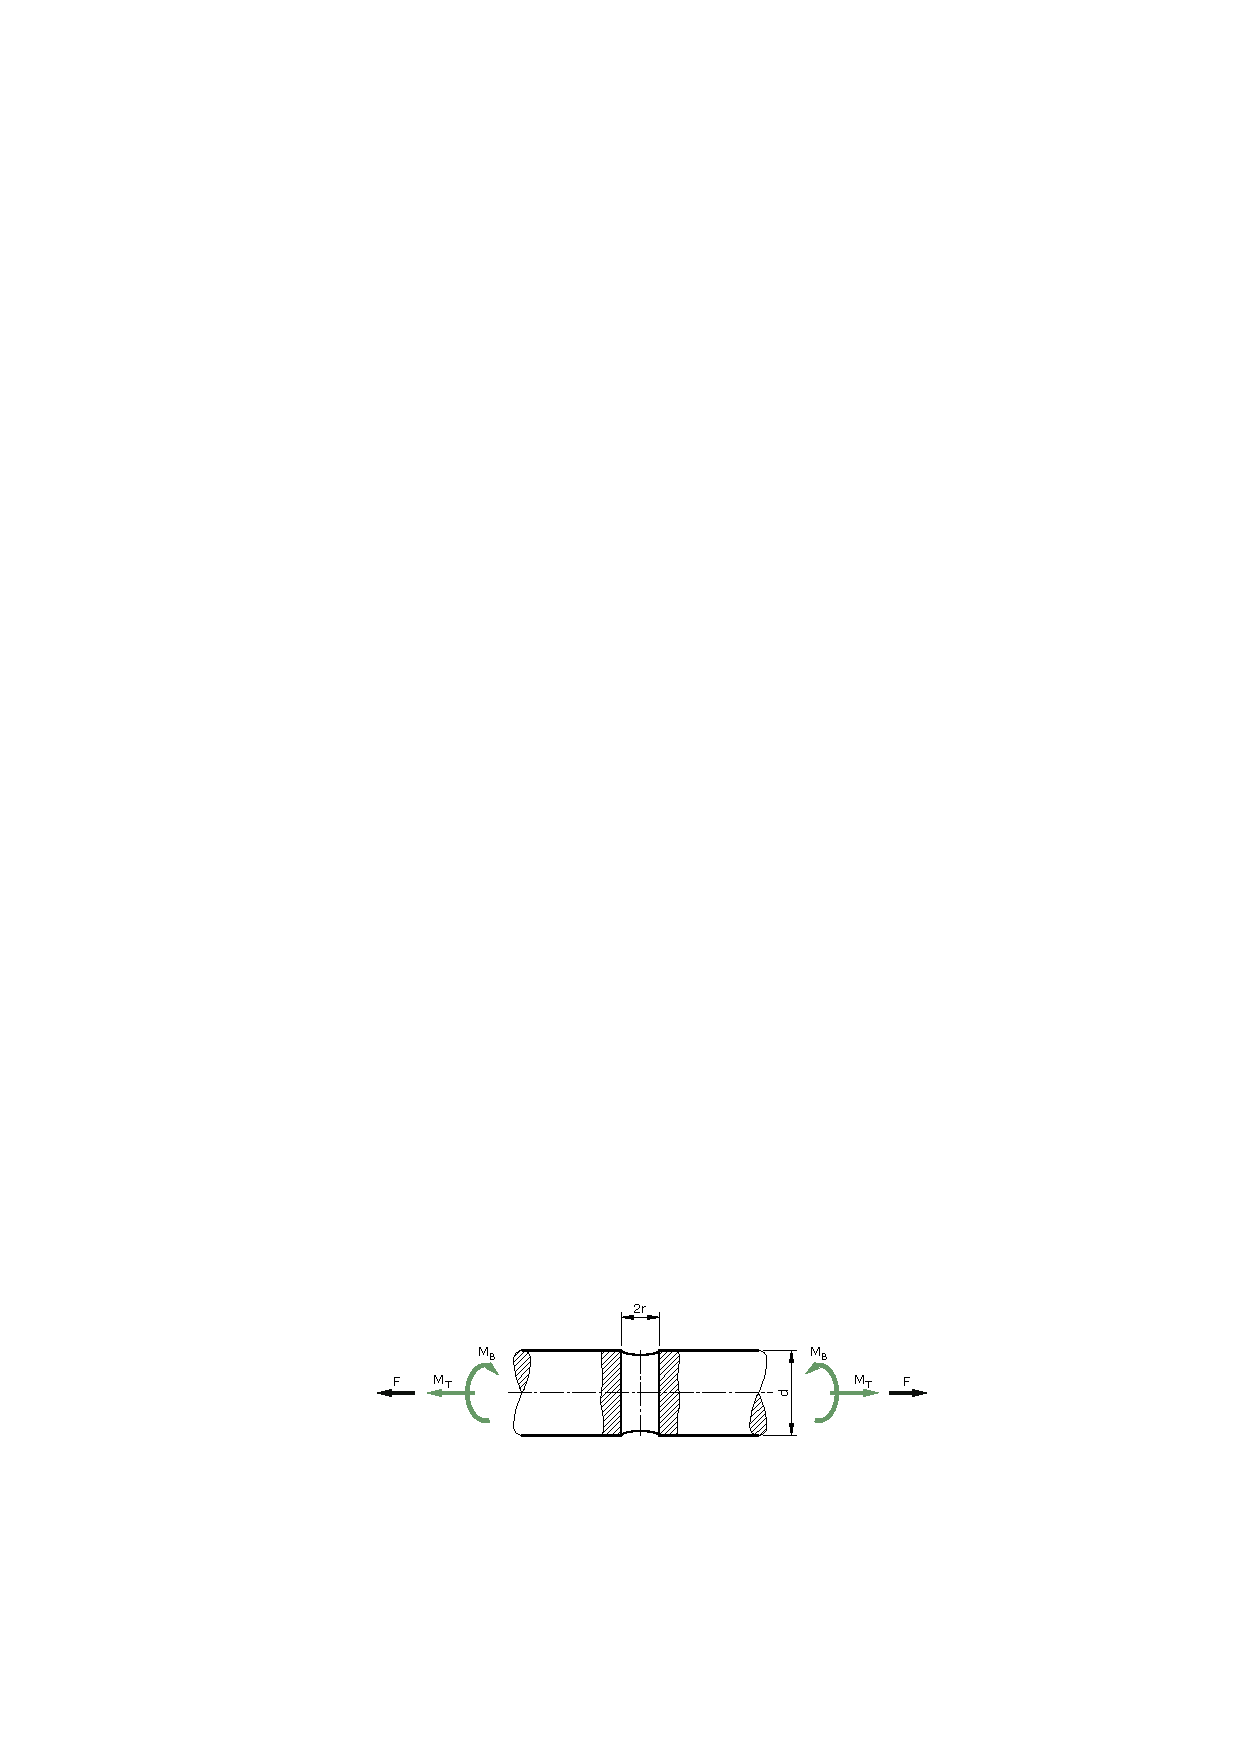
\includegraphics[width=\columnwidth]{graphics/rundstab_querbohrung}
		\begin{align*}
			\alpha_{\sigma\text{Zug}} &= 3 - \frac{2r}{d} \\
			\alpha_{\sigma\text{Bieg}} &= 1.4 \left( \frac{2r}{d}\right) + 3 - 2.8\cdot \sqrt{\frac{2r}{d}} \\
			\alpha_{\tau} &= 2.023 - 1.125\cdot\sqrt{\frac{2r}{d}}
		\end{align*}
	% subsection: Formzahl für Rundstab mit Querbohrung (end)
% section: Formzahl (end)
\section{Örtliche Überschreitung der Fliessgrenze} % (fold)
	Bei Beuteilen mit \emph{Lüdersdehnung} verbleibt nach erster Plastifizierung im entspannten Zustand eine geringe \emph{Druckspannung} in Kerbgrund. Bei erneuter identischer Belastung wird die Fliessgrenze nicht mehr überschritten.
% section: Örtliche Überschreitung der Fliessgrenze (end)
\section{Kerb-Einfluss-Überlagerung} % (fold)
	Bei zwei sich überlagernden Kerbwirkungen gilt für die resultierende Formzahl:
	\begin{equation*}
		\alpha = \alpha_1 \cdot \alpha_2
	\end{equation*}
% section: Kerb-Einfluss-Überlagerung (end)
\section{Einfluss der Kerbwirkung auf die Festigkeitsrechnung} % (fold)
	\subsection{Ruhende Belastung, zähes Material} % (fold)
		Spannungsspitzen infolge Kerbwirkung werden \emph{nicht} be\-rück\-sich\-tigt (Gestaltänderungs- oder Schubspannungshypothese).
		\begin{equation*}
			\sigma_V = \sqrt{(\sigma_{\text{x,Zug,n}} + \sigma_{\text{x,Bieg,n}})^2 + 3 \tau_{\text{t,n}}^2}
		\end{equation*}
	% subsection: Ruhende Belastung, zähes Material (end)
	\subsection{Ruhende Belastung, sprödes Material} % (fold)
		Spannungsspitzen ergeben Rissbildung, daher \emph{muss} mit den maximalen Spannungsspitzen im Kerbgrund dimensioniert werden (Normalspannungshypothese).
		\begin{align*}
			\sigma_V =&\: \half  \parens{\alpha_{\sigma\text{Zug}}\sigma_{\text{x,Zug,n}} + \alpha_{\sigma\text{Bieg}}\sigma_{\text{x,Bieg,n}}} \\
			&+ \frac{1}{2}\sqrt{(\alpha_{\sigma\text{Zug}}\sigma_{\text{x,Zug,n}} + \alpha_{\sigma\text{Bieg}}\sigma_{\text{x,Bieg,n}})^2+4(\alpha_{\tau}\tau_t)^2}
		\end{align*}
	% subsection: Ruhende Belastung, sprödes Material (end)
	\subsection{Wechselnde Belastung} % (fold)
		Kerbeinflüsse \emph{müssen} berücksichtigt werden. Siehe Kapitel~\ref{chap:ermuedungsfestigkeit}~\nameref{chap:ermuedungsfestigkeit} auf Seite~\pageref{chap:ermuedungsfestigkeit}.
	% subsection: Wechselnde Belastung (end)
% section: Einfluss der Kerbwirkung auf die Festigkeitsrechnung (end)
\section{Gestaltungsrichtlinien} % (fold)
	\begin{tightitemize}
		\item Möglichst gradlinige Kraftflüsse auf kurzen Wegen
		\item Kerben verhindern
		\item Notwendige Kerben in ihrer Wirkung abschwächen
	\end{tightitemize}
	
	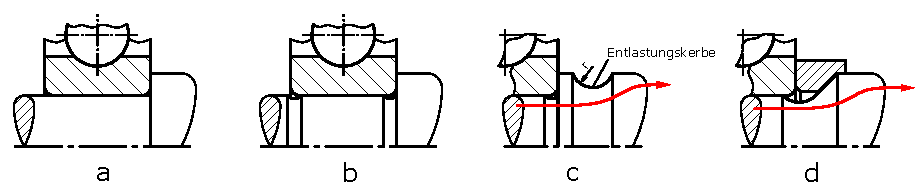
\includegraphics[width=\columnwidth]{graphics/kerben}
	\begin{itemize}
		\item[a:] Aufgezogenes Wälzlager mit kleinem Rundungsradius (schlechte Lösung)
		\item[b:] Vergrösserte Ausrundung des Wellenabsatzes
		\item[c:] Zusätzliche Entlastungskerbe
		\item[d:] Vergrösserte Ausrundung und konischer Übergang mit Stützring
	\end{itemize}
% section: Gestaltungsrichtlinien (end)